% Created 2020-07-20 lun 12:34
% Intended LaTeX compiler: pdflatex
\documentclass[presentation,aspectratio=169]{beamer}
\usepackage[utf8]{inputenc}
\usepackage[T1]{fontenc}
\usepackage{graphicx}
\usepackage{grffile}
\usepackage{longtable}
\usepackage{wrapfig}
\usepackage{rotating}
\usepackage[normalem]{ulem}
\usepackage{amsmath}
\usepackage{textcomp}
\usepackage{amssymb}
\usepackage{capt-of}
\usepackage{hyperref}
\usepackage{khpreamble}
\usepackage{amssymb}
\usepackage{pgfplotstable}
\DeclareMathOperator{\shift}{q}
\DeclareMathOperator{\diff}{p}
\usetheme{default}
\author{Kjartan Halvorsen}
\date{\today}
\title{Control computarizado - Identificación de sistemas}
\hypersetup{
 pdfauthor={Kjartan Halvorsen},
 pdftitle={Control computarizado - Identificación de sistemas},
 pdfkeywords={},
 pdfsubject={},
 pdfcreator={Emacs 26.3 (Org mode 9.3.6)}, 
 pdflang={English}}
\begin{document}

\maketitle

\section{Retroalimentación, Tarea 2 - PID discretos}
\label{sec:org9170d1d}

\begin{frame}[label={sec:org340d883}]{Retroalimentación -  Tarea 2}
\begin{itemize}
\item Más variedad en nivel del trabajo esta vez
\item Bastante retador
\item Gráficas con referencia a fuente
\end{itemize}
\end{frame}

\begin{frame}[label={sec:org18f94a3}]{Discretización}
\begin{columns}
\begin{column}{0.65\columnwidth}
\alert{Actividad} Aplica el método de Tustin
\[ z = \mathrm{e}^{sh} = \frac{\mathrm{e}^{sh/2}}{\mathrm{e}^{-sh/2}} \approx \frac{ 1 + \frac{sh}{2}}{1 - \frac{sh}{2}}\]
\[ s = \frac{2}{h} \cdot \frac{z-1}{z+1}\]
para discretizar el controlador PD ideal
\[F_{PD}(s) = K\big(1 + sT_d\big).\]
Marca (aproximadamente) el cero y el polo en el plano z 
\end{column}
\begin{column}{0.35\columnwidth}
\begin{center}
  \begin{tikzpicture}[scale=1.6]
    \draw[->] (-1.5, 0) -- (1.5, 0) node[below] {Re};
    \draw[->] (0,-1.50) -- (0,1.5) node[left] {Im};

    \draw[domain=0:360, samples=361, dashed] plot ({cos(\x)}, {sin(\x)});
    \node at (1,-0.2) {1};

  \end{tikzpicture}
\end{center}
\end{column}
\end{columns}
\end{frame}




\begin{frame}[label={sec:orgb490c71}]{Ganancia del PD ideal}
\begin{columns}
\begin{column}{0.65\columnwidth}
En tiempo discreto el diagrama de Bode de una función de transferencia nos da los valores de esta función evaluada por puntos en el semicirculo arriba del circulo unitario en el plano z. Es decir
\[F_{PD}(\mathrm{e}^{i\omega h}), \quad 0 \le \omega h \le \pi \]
\alert{Actividad} Que pasa con la ganancia del PD discretizado con el método de Tustin \[|F_{PD}(z)| = \left | \frac{z(1 + \frac{2T_d}{h}) - (\frac{2T_d}{h}-1)}{z + 1} \right|\]
cuando \(\omega = \omega_N = \frac{\pi}{h}\)?
\end{column}
\begin{column}{0.35\columnwidth}
\begin{center}
  \begin{tikzpicture}[scale=1.4]
    \draw[->] (-1.5, 0) -- (1.5, 0) node[below] {Re};
    \draw[->] (0,-1.50) -- (0,1.5) node[left] {Im};

    \draw[domain=0:360, samples=361, dashed] plot ({cos(\x)}, {sin(\x)});
    \node at (1,-0.2) {1};

    \draw[domain=0:180, samples=181, red, thick] plot ({cos(\x)}, {sin(\x)});

    \node[coordinate, pin=60:{$\omega = \frac{\pi}{2h}$}] at (0,1);
    \node[coordinate, pin=150:{$\omega = \frac{\pi}{h}$}] at (-1,0);

  \end{tikzpicture}
\end{center}
\end{column}
\end{columns}
\end{frame}

\section{Intro}
\label{sec:org46be661}
\begin{frame}[label={sec:org0a68327}]{Identificación de sistemas}
\end{frame}

\begin{frame}[label={sec:orga68fad4}]{Un proceso complejo}
\begin{columns}
\begin{column}{0.6\columnwidth}
From Wikipedia "Cyclonic separation"
\end{column}
\begin{column}{0.4\columnwidth}
\begin{center}
\includegraphics[height=1.0\textheight]{../../figures/Vertical-cyclone.jpg}
\end{center}
\end{column}
\end{columns}
\end{frame}

\begin{frame}[label={sec:orga83c13d}]{Identificación de sistemas}
\begin{center}
  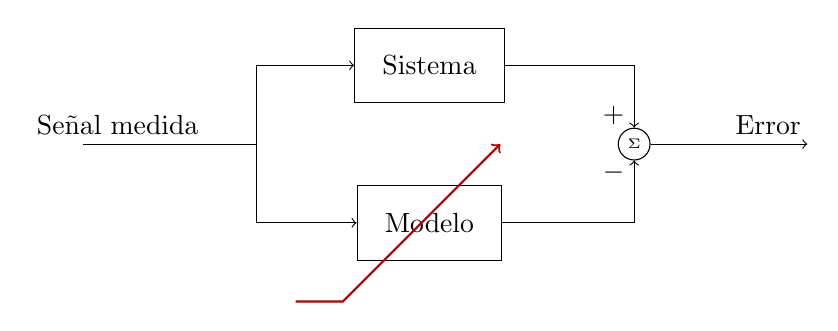
\begin{tikzpicture}[node distance=22mm, block/.style={rectangle, draw, minimum width=15mm, inner sep=10pt}, sumnode/.style={circle, draw, inner sep=2pt},]

    \node[coordinate] (input) {};
    \node[coordinate, right of=input] (copy) {};
    \node[coordinate, right of=copy] (midp) {};
    \node[block, above of=midp, node distance=10mm] (sys)  {Sistema};
    \node[block, below of=midp, node distance=10mm] (mod)  {Modelo};
    \node[sumnode, right of=midp, node distance=26mm] (sum) {\tiny $\Sigma$};
    \node[coordinate, right of=sum, node distance=22mm] (output) {};

    \draw[-] (input) -- node[above, pos=0.2] {Señal medida} (copy);
    \draw[->] (copy) |- node[above] {} (sys);
    \draw[->] (copy) |- node[above] {} (mod);
    \draw[->] (sys) -| node[left, pos=0.9] {$+$} (sum);
    \draw[->] (mod) -| node[left, pos=0.9] {$-$} (sum);
    \draw[->] (sum) -- node[above, near end] {Error} (output);

    \draw[thick, red!70!black, ->] (2.7,-2) -- (3.3,-2) -- (5.3, 0);
  \end{tikzpicture}
\end{center}
\end{frame}

\begin{frame}[label={sec:org16fe05a}]{Ajustando un modelo - regresión lineal}
\begin{columns}
\begin{column}{0.4\columnwidth}
\alert{Objetivo} Dado observaciones \[\mathcal{D} = \{ (x_1,y_1), (x_2, y_2), \ldots, (x_N, y_N)\}\] y 
modelo \(\mathcal{M}: \; y = ax + b  + e\), obtiene los parametros \((a,b)\) que da el modelo que mejor se ajuste a los datos.

El término de ruido, o error, \(e\), incluye errores de modelación y perturbaciones.
\end{column}
\begin{column}{0.6\columnwidth}
\begin{center}
\includegraphics[height=0.6\textheight]{lsq-example}
\end{center}
\end{column}
\end{columns}
\end{frame}


\begin{frame}[label={sec:org784f37f}]{Ajustando un modelo - regresión lineal}
Dado observaciones \(\mathcal{D} = \{ (x_1,y_1), (x_2, y_2), \ldots, (x_N, y_N)\}\) y 
modelo \(\mathcal{M}: \; y = ax + b  + e\). 

\begin{columns}
\begin{column}{0.7\columnwidth}
La predicción es
\[ \hat{y_k} = ax_k + b = \underbrace{\begin{bmatrix} x & 1 \end{bmatrix}}_{\varphi_k^T} \underbrace{\begin{bmatrix} a\\b\end{bmatrix}}_{\theta}\]
y el error de predicción 
\[ \epsilon_k = y_k - \hat{y}_k = y_k - ax_k-b = y - \varphi_k^T\theta.\]

Buscamos parametros \(\theta^T = \begin{bmatrix} a & b \end{bmatrix}\) que minimiza
 la función de pérdida \[J(\theta) =  \sum_{k=1}^N g\big(\epsilon_k\big).\]
\end{column}

\begin{column}{0.3\columnwidth}
\begin{center}
\includegraphics[height=0.4\textheight]{lsq-example}
\end{center}
\end{column}
\end{columns}
\end{frame}


\begin{frame}[label={sec:org117654a}]{Ajustando un modelo - regresión lineal}
Dado observaciones \(\mathcal{D} = \{ (x_1,y_1), (x_2, y_2), \ldots, (x_N, y_N)\}\) y 
modelo \(\mathcal{M}: \; y = ax + b  + e\). 

\begin{columns}
\begin{column}{0.6\columnwidth}
La función de pérdida más común es \alert{mínimos cuadrados}

\begin{align*}
\hat{\theta}_{LS} &= \arg\min J_{LS}(\theta) = \arg\min \sum_{k=1}^N \epsilon_k^2\\
&= \arg\min \sum_{k=1}^N (y_k - \hat{y}_k)^2 
= \arg\min \sum_{k=1}^N (y_k - \varphi_k\T\theta)^2\\ 
&= \arg\min \sum_{k=1}^N (y_k - ax_k - b)^2
\end{align*}
\end{column}

\begin{column}{0.4\columnwidth}
\begin{center}
\includegraphics[height=0.5\textheight]{lsq-example}
\end{center}
\end{column}
\end{columns}
\end{frame}



\begin{frame}[label={sec:orgc6e7f56}]{El problema con mínimos cuadrados}
\begin{columns}
\begin{column}{0.4\columnwidth}
\begin{align*}
 \text{minimiza} \; &\sum_k g(\epsilon_k)\\
 \text{dónde} \; g(u) &= u^2
\end{align*}
\end{column}

\begin{column}{0.6\columnwidth}
\begin{center}
  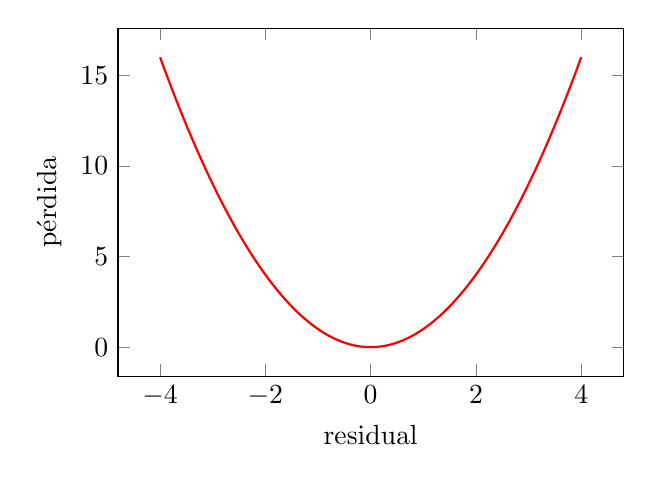
\begin{tikzpicture}
    \begin{axis}[
      width=8cm,
      height=6cm,
      ylabel=pérdida,
      xlabel=residual,
      ]
      \addplot[red, thick, no marks, domain=-4:4, samples=201] {x^2};
    \end{axis}
  \end{tikzpicture}
\end{center}
\end{column}
\end{columns}
\end{frame}

\begin{frame}[label={sec:orgffafbca}]{Más robusta: La función de pérdida de Huber}
\begin{columns}
\begin{column}{0.4\columnwidth}
También conocido como \alert{regresión robusta}
\begin{align*}
 \text{minimiza} \; &\sum_k g_{hub}(\epsilon_k)\\
 \text{dónde}\; g_{hub}(u) &= \begin{cases} u^2 & |u| \le M\\ M(2|u|-M) & |u| > M \end{cases}
\end{align*}
\end{column}

\begin{column}{0.6\columnwidth}
\begin{center}
  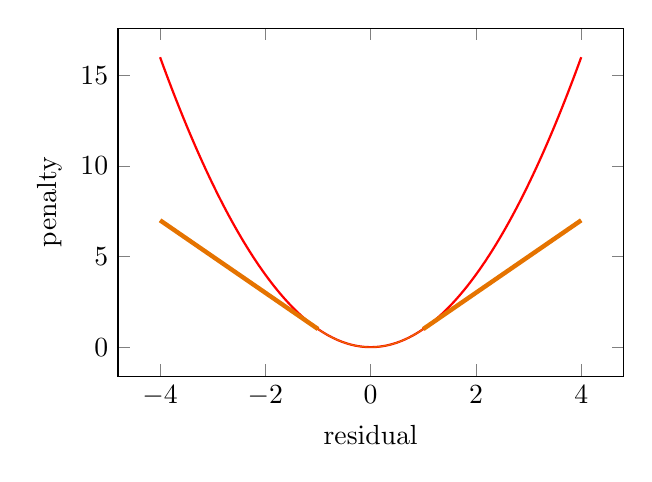
\begin{tikzpicture}
    \begin{axis}[
      width=8cm,
      height=6cm,
      ylabel=penalty,
      xlabel=residual,
      ]
      \addplot[red, thick, no marks, domain=-4:4, samples=201] {x^2};
      \addplot[orange!90!black, ultra thick, no marks, domain=-4:-1, samples=201] {2*abs(x)-1};
      \addplot[orange!90!black, thin, no marks, domain=-1:1, samples=201] {x^2};
      \addplot[orange!90!black, ultra thick, no marks, domain=1:4, samples=201] {2*abs(x)-1};
    \end{axis}
  \end{tikzpicture}
\end{center}
\end{column}
\end{columns}
\end{frame}

\section{AR-model}
\label{sec:orga00114e}

\begin{frame}[label={sec:org3a7ba52}]{Ejemplo - Modelo autoregresivo (AR)}
\end{frame}
\begin{frame}[label={sec:orga436dbc}]{Modelo autoregresivo (AR)}
Dado una secuencia discreta observada \(y(k), \; k=1,2,\ldots,N\), y el modelo autoregresivo
\[ y(k+1) = -ay(k) + e(k+1),\]
dónde \(e(k)\) es una sequencia discreta de ruido blanco.

\alert{Objetivo} Estimar el parametro \(a\).

\begin{enumerate}
\item Forma el predictor de un paso adelante \[\hat{y}_{k+1} = -ay_k=-y_ka = \varphi_{k+1} \theta,\] y el error de predicción \[\epsilon_k = y_k - \hat{y}_k = y_k - \varphi_k \theta\]
\end{enumerate}
\end{frame}


\begin{frame}[label={sec:orga296681}]{Modelo autoregresivo (AR)}
Dado una secuencia discreta observada \(y(k), \; k=1,2,\ldots,N\), y el modelo autoregresivo
\(y(k+1) = -ay(k) + e(k+1),\)
dónde \(e(k)\) es una sequencia discreta de ruido blanco.

\alert{Objetivo} Estimar el parametro \(a\).

\begin{enumerate}
\setcounter{enumi}{1}
\item Reune todas las observaciónes \(y_k\) y predicciones \(\hat{y}_k\) en forma vectoral
\begin{align*}
\epsilon &= \begin{bmatrix} \epsilon_2\\\epsilon_2\\\vdots\\\epsilon_N\end{bmatrix} =  \begin{bmatrix} y_2\\ y_3\\\vdots\\y_N \end{bmatrix} - \begin{bmatrix} \hat{y}_2\\ \hat{y}_3\\\vdots\\\hat{y}_N \end{bmatrix}
 =  \begin{bmatrix} y_2\\ y_3\\\vdots\\y_N \end{bmatrix} - \begin{bmatrix} -y_1 a\\ -y_2 a\\\vdots\\-y_{N-1}^T\theta \end{bmatrix} =  \begin{bmatrix} y_2\\ y_3\\\vdots\\y_N \end{bmatrix} - \begin{bmatrix} \varphi_2^T\theta\\ \varphi_3^T\theta\\\vdots\\\varphi_N^T\theta \end{bmatrix}\\
&= y - \underbrace{\begin{bmatrix}\varphi_1^T\\\varphi_2^T\\\vdots\\\varphi_N^T\end{bmatrix}}_{\Phi}\theta = y - \Phi\theta 
\end{align*}
\end{enumerate}
\end{frame}



\begin{frame}[label={sec:orga16749f}]{Modelo autoregresivo (AR)}
Dado una secuencia discreta observada \(y(k), \; k=1,2,\ldots,N\), y el modelo autoregresivo
\(y(k+1) = -ay(k) + e(k+1),\)
dónde \(e(k)\) es una sequencia discreta de ruido blanco.

\alert{Objetivo} Estimar el parametro \(a\).

\begin{enumerate}
\setcounter{enumi}{2}
\item Obtiene el estimado de mínimos cuadrados 
\begin{align*}
 \theta_{LS} &= (\Phi^T\Phi)^{-1}\Phi^T y\\ &= \left(\begin{bmatrix} -y_1 & -y_2 & \cdots & -y_{N-1}\end{bmatrix}\begin{bmatrix}-y_1\\-y_2\\\vdots\\-y_{N-1}\end{bmatrix}\right)^{-1}\begin{bmatrix} -y_1 & -y_2 & \cdots & -y_{N-1}\end{bmatrix}\begin{bmatrix}y_2\\y_3\\\vdots\\y_N\end{bmatrix}\\
 &= -\frac{\sum_{k=1}^{N-1} y_ky_{k+1}}{\sum_{k=1}^{N-1}y_k^2}
 \end{align*}
\end{enumerate}
\end{frame}


\begin{frame}[label={sec:org7516c15},fragile]{Computación de la solución de mínimos cuadrados}
 Dado error de predicción en forma vectoral para sistema de orden \(n\)
\(\epsilon = y - \Phi\theta\). Forma el sistema de ecuaciones
\begin{align*}
\Phi \theta &= y\\
\begin{bmatrix}\varphi_{n+1}^T\\\varphi_{n+2}^T\\\varphi_{n+3}^T\\\varphi_{n+4}^T\\\vdots\\\varphi_{N}^T\end{bmatrix} \begin{bmatrix}\theta_1\\\theta_2\\\vdots\\\theta_m\end{bmatrix} &= \begin{bmatrix}y_{n+1}\\y_{n+2}\\y{n+3}\\y_{n+4}\\\vdots\\ y_{N}\end{bmatrix}
\end{align*}
Resuelva las ecuaciones usando métodos numericamente robustos de algebra lineal, por ejemplo   factorización L-U. En matlab se escribe
\begin{verbatim}
theta_LS = Phi \ y
\end{verbatim}
\end{frame}

\begin{frame}[label={sec:orge77fb68}]{Ejemplo numerico}
\href{https://mybinder.org/v2/gh/kjartan-at-tec/mr2007-computerized-control/master?filepath=.\%2Fsystem-identification\%2Fnotebooks\%2FAR-example.ipynb}{Mybinder}
\end{frame}



\begin{frame}[label={sec:org0fd8c5c}]{Model AR de orden \(n\)}
Dado una secuencia discreta observada \(y(k), \; k=1,2,\ldots,N\), y el modelo autoregresivo
\begin{align*} 
A(z)Y(z) = z^nE(z) \quad \Leftrightarrow \quad A(\shift)y(k) &= \shift^{n-1} e(k)\\
(\shift^n + a_1\shift^{n-1} + a_2\shift^{n-2} + \cdots + a_n)y(k) &= \shift^n e(k)\\
(\shift + a_1 + a_2\shift{-1} + \cdots + a_n\shift^{-n+1})y(k) &= \shift e(k)\\
y(k+1) + a_1y(k)  + a_2y(k-1) + \cdots + a_ny(k-n+1) &= e(k+1)\\
y(k+1) = -a_1y(k)  - a_2y(k-1) - \cdots - a_ny(k-n+1) &+ e(k+1)
\end{align*}
dónde \(e(k)\) es una sequencia discreta de ruido blanco.

\alert{Objetivo} Estimar los parametro \(a_1, a_2, \ldots, \a_n\).
\end{frame}


\begin{frame}[label={sec:org30596ce}]{Model AR de orden \(n\)}
Dado una secuencia discreta observada \(y(k), \; k=1,2,\ldots,N\), y el modelo autoregresivo
\(y(k+1) = -a_1y(k)  - a_2y(k-1) - \cdots - a_ny(k-n+1) + e(k+1)\).

\begin{enumerate}
\item Forma el predictor de un paso adelante 
\[\hat{y}_{k+1} = -a_1y_k-a_2y_{k-1} - \ldots - a_n y_{k-n+1}a = \underbrace{\begin{bmatrix} -y_{k} & -y_{k-1} & \cdots & -y_{k-n+1}\end{bmatrix}}_{\varphi_{k+1}^T}\underbrace{\begin{bmatrix}a_1\\a_2\\\vdots\\a_n\end{bmatrix}}_{\theta}\]
y el error de predicción \[\epsilon_k = y_k - \hat{y}_k = y_k - \varphi_k^T \theta\]
\end{enumerate}
\end{frame}

\begin{frame}[label={sec:org9107234}]{Model AR de orden \(n\)}
Dado una secuencia discreta observada \(y(k), \; k=1,2,\ldots,N\), y el modelo autoregresivo
\(y(k+1) = -a_1y(k)  - a_2y(k-1) - \cdots - a_ny(k-n+1) + e(k+1)\).

\begin{enumerate}
\setcounter{enumi}{1}
\item Reune todas las observaciónes \(y_k\) y predicciones \(\hat{y}_k\) en forma vectoral
\begin{align*}
\epsilon &= \begin{bmatrix} \epsilon_{n+1}\\\epsilon_{n+2}\\\vdots\\\epsilon_N\end{bmatrix} =  \begin{bmatrix} y_{n+1}\\ y_{n+2}\\\vdots\\y_N \end{bmatrix} - \begin{bmatrix} \hat{y}_{n+1}\\ \hat{y}_{n+2}\\\vdots\\\hat{y}_N \end{bmatrix}
 =  \begin{bmatrix} y_{n+1}\\ y_{n+2}\\\vdots\\y_N \end{bmatrix} - \begin{bmatrix} \varphi_{n+1}^T\theta\\ \varphi_{n+2}^T\theta\\\vdots\\\varphi_N^T\theta \end{bmatrix}\\
&= y - \underbrace{\begin{bmatrix}\varphi_{n+1}^T\\\varphi_{n+2}^T\\\vdots\\\varphi_N^T\end{bmatrix}}_{\Phi}\theta = y - \Phi\theta 
\end{align*}
\end{enumerate}
\end{frame}

\begin{frame}[label={sec:org8ece0af}]{Model AR de orden \(n\)}
Dado una secuencia discreta observada \(y(k), \; k=1,2,\ldots,N\), y el modelo autoregresivo
\(y(k+1) = -a_1y(k)  - a_2y(k-1) - \cdots - a_ny(k-n+1) + e(k+1)\).
\begin{enumerate}
\setcounter{enumi}{2}
\item Obtiene el estimado de mínimos cuadrados, que es
\begin{align*}
 \theta_{LS} &= (\Phi^T\Phi)^{-1}\Phi^T y
 \end{align*}
formando y resolviendo el sistema de ecuaciones
\begin{align*}
\Phi \theta &= y\\
\begin{bmatrix}\varphi_{n+1}^T\\\varphi_{n+2}^T\\\varphi_{n+3}^T\\\varphi_{n+4}^T\\\vdots\\\varphi_{N}^T\end{bmatrix} \begin{bmatrix}a_1\\a_2\\\vdots\\a_n\end{bmatrix} &= \begin{bmatrix}y_{n+1}\\y_{n+2}\\y_{n+3}\\y_{n+4}\\\vdots\\ y_{N}\end{bmatrix}
\end{align*}
\end{enumerate}
\end{frame}


\begin{frame}[label={sec:org52b3538}]{Modelo autoregresivo (AR) - Ejercicio}
Dado una secuencia discreta observada \(y(k), \; k=1,2,\ldots,N\), y el modelo autoregresivo de segunda orden
\[ y(k+2) + a_1y(k+1) + a_2y(k) = e(k+2),\]
dónde \(e(k)\) es una sequencia discreta de ruido blanco.

\alert{Actividad} Forma las ecuaciones \[ \Phi \theta = y\]
\end{frame}


\section{ARX-model}
\label{sec:orgf051171}

\begin{frame}[label={sec:orgde27b90}]{Model AutoRegresivo con variables eXógenas (ARX)}
Dado señal discreta de entrada de un sistema \(u(k), \; k=1,2,\ldots, N\) y observaciones de la respuesta \(y(k), \; k=1,2,\ldots,N\), y el modelo ARX
\[ A(\shift) y(k) = B(\shift)u(k) + e(k+n),\]
dónde \(e(k)\) es una sequencia discreta de ruido blanco.

\alert{Actividad} Llena los bloques

\begin{center}
  \begin{tikzpicture}[node distance=22mm, block/.style={rectangle, draw, minimum width=15mm, minimum height=12mm}, sumnode/.style={circle, draw, inner sep=2pt}]
    
    \node[coordinate] (input) {};
    \node[block, right of=input, node distance=20mm] (plant)  {};
    \node[sumnode, right of=plant, node distance=24mm] (sum) {\tiny $\Sigma$};
    \node[block, above of=sum, node distance=20mm] (dist)  {};

    \node[coordinate, above of=dist, node distance=12mm] (disturbance) {};
    \node[coordinate, right of=sum, node distance=20mm] (output) {};

    \draw[->] (input) -- node[above, pos=0.3] {$u(k)$} (plant);
    \draw[->] (plant) -- node[above] {} (sum);
    \draw[->] (sum) -- node[above, near end] {$y(k)$} (output);
    \draw[->] (disturbance) -- node[right, pos=0.2] {$e(k)$} (dist);
    \draw[->] (dist) -- node[above] {} (sum);

  \end{tikzpicture}
\end{center}
\end{frame}
\end{document}